\chapter{Números Naturais E Inteiros}


\section{Sistemas de numeração}

A televisão, o computador e os demais objetos que costumamos utilizar diariamente não surgiram do nada, foram criados por pessoas como nós que, por seus motivos, as fizeram. Com as ideias ocorre o mesmo. Se hoje se torna absurdo que uma pessoa seja considerada dona de outra foi por que alguém cultivou essa ideia e lutou para que fosse disseminada ao ponto que hoje em dia se torna absurdo a escravisão.

O sistema de numeração é uma ideia muito elaborada e extremamente útil que foi construido vagarosamente por diversos povos para solucionárem suas dificuldades e facilitarem suas vidas. Não é necessário conhecer como uma televisão é feita para poder asistíla, logo normalmente não é necessário conhecer a história do desenvolvimento dos sistemas numéricos para poder utilizá-los na hora de calcular o troco do pão. Porém conhecer como a TV funciona pode ajudar bastante na hora de solucionar pequenos problemas economisando com um serviço especializado. Pode-se ainda procurar meios para evoluir a televisão para que ela seja mais útil e tenha mais funcionalidades. Igualmente conhecer melhor os sistemas de numeração é essencial para poder absorver e melhorar sua forma de lhedar com os números.

Vamos a uma curiosidade. Qual é o valor representado por dois tracinhos verticais? Se for no sistema binário valerá 3, se for no romano será 2, caso seja no decimal derá 11. O mesmo símbolo pode representar coisas diferentes em contextos diferentes.

%http://esj.eti.br/CEFETMG/Disciplinas/PC1/PC1_Unidade_02.pdf
%@article{junior2011sistemas,
%  title={Sistemas de Numera{\c{c}}{\~a}o},
%  author={J{\'u}nior, Edwar Saliba},
%  year={2011}
%}




\section{Números Naturais como notação}
\subsection{Classificação de Livros e Documentos}

\begin{center}
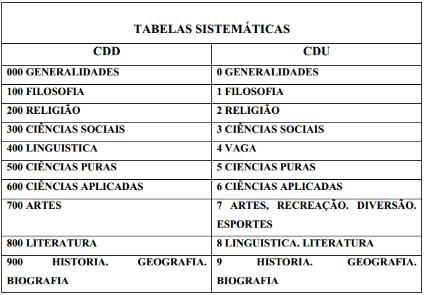
\includegraphics[scale=.9]{./imagens/19.jpg}
\end{center}



